\begin{problem}
  {Q4(a)}
  What is the value of the $s-t$ flow depicted in figure 7.26? Is this a maximum $(s,t)$ flow in this graph? The figure is reproduced below with additional node labels.
  \begin{center}
  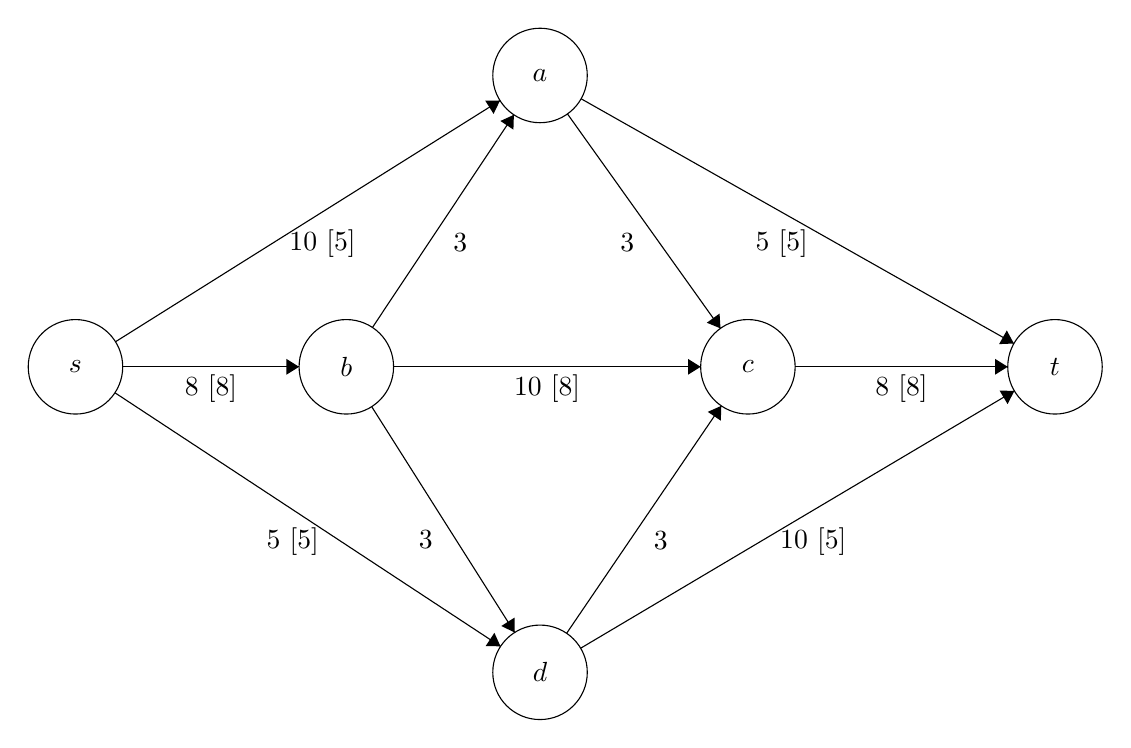
\begin{tikzpicture}[scale=0.2]
  \tikzstyle{every node}+=[inner sep=0pt]
  \draw [black] (7.3,-27.8) circle (3);
  \draw (7.3,-27.8) node{$s$};
  \draw [black] (36.8,-9.3) circle (3);
  \draw (36.8,-9.3) node{$a$};
  \draw [black] (24.5,-27.8) circle (3);
  \draw (24.5,-27.8) node{$b$};
  \draw [black] (36.8,-47.2) circle (3);
  \draw (36.8,-47.2) node{$d$};
  \draw [black] (50,-27.8) circle (3);
  \draw (50,-27.8) node{$c$};
  \draw [black] (69.5,-27.8) circle (3);
  \draw (69.5,-27.8) node{$t$};
  \draw [black] (9.84,-26.21) -- (34.26,-10.89);
  \fill [black] (34.26,-10.89) -- (33.32,-10.9) -- (33.85,-11.74);
  \draw (22.99,-19.05) node [below] {$10~[5]$};
  \draw [black] (9.81,-29.45) -- (34.29,-45.55);
  \fill [black] (34.29,-45.55) -- (33.9,-44.69) -- (33.35,-45.53);
  \draw (21.1,-38) node [below] {$5~[5]$};
  \draw [black] (10.3,-27.8) -- (21.5,-27.8);
  \fill [black] (21.5,-27.8) -- (20.7,-27.3) -- (20.7,-28.3);
  \draw (15.9,-28.3) node [below] {$8~[8]$};
  \draw [black] (27.5,-27.8) -- (47,-27.8);
  \fill [black] (47,-27.8) -- (46.2,-27.3) -- (46.2,-28.3);
  \draw (37.25,-28.3) node [below] {$10~[8]$};
  \draw [black] (53,-27.8) -- (66.5,-27.8);
  \fill [black] (66.5,-27.8) -- (65.7,-27.3) -- (65.7,-28.3);
  \draw (59.75,-28.3) node [below] {$8~[8]$};
  \draw [black] (26.16,-25.3) -- (35.14,-11.8);
  \fill [black] (35.14,-11.8) -- (34.28,-12.19) -- (35.11,-12.74);
  \draw (31.26,-19.88) node [right] {$3$};
  \draw [black] (26.11,-30.33) -- (35.19,-44.67);
  \fill [black] (35.19,-44.67) -- (35.19,-43.72) -- (34.34,-44.26);
  \draw (30.02,-38.8) node [left] {$3$};
  \draw [black] (38.54,-11.74) -- (48.26,-25.36);
  \fill [black] (48.26,-25.36) -- (48.2,-24.42) -- (47.39,-25);
  \draw (42.81,-19.92) node [left] {$3$};
  \draw [black] (38.49,-44.72) -- (48.31,-30.28);
  \fill [black] (48.31,-30.28) -- (47.45,-30.66) -- (48.28,-31.22);
  \draw (44,-38.85) node [right] {$3$};
  \draw [black] (39.41,-10.78) -- (66.89,-26.32);
  \fill [black] (66.89,-26.32) -- (66.44,-25.49) -- (65.95,-26.36);
  \draw (52.15,-19.05) node [below] {$5~[5]$};
  \draw [black] (39.38,-45.67) -- (66.92,-29.33);
  \fill [black] (66.92,-29.33) -- (65.98,-29.31) -- (66.49,-30.17);
  \draw (54.15,-38) node [below] {$10~[5]$};
  \end{tikzpicture}
  \end{center}
  \noindent
  $v(f) = 18$, this is not a maximum flow. \\
  There exists, trivially, a flow of higher value shown below. \\
  \begin{center}
  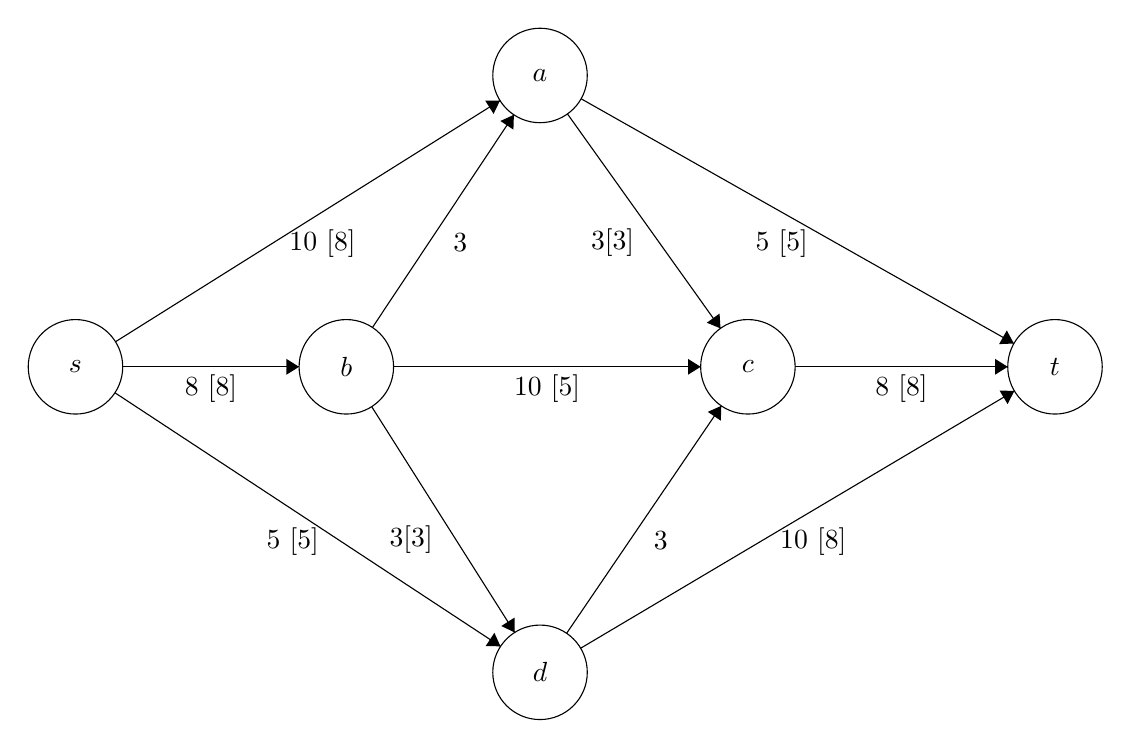
\begin{tikzpicture}[scale=0.2]
  \tikzstyle{every node}+=[inner sep=0pt]
  \draw [black] (7.3,-27.8) circle (3);
  \draw (7.3,-27.8) node{$s$};
  \draw [black] (36.8,-9.3) circle (3);
  \draw (36.8,-9.3) node{$a$};
  \draw [black] (24.5,-27.8) circle (3);
  \draw (24.5,-27.8) node{$b$};
  \draw [black] (36.8,-47.2) circle (3);
  \draw (36.8,-47.2) node{$d$};
  \draw [black] (50,-27.8) circle (3);
  \draw (50,-27.8) node{$c$};
  \draw [black] (69.5,-27.8) circle (3);
  \draw (69.5,-27.8) node{$t$};
  \draw [black] (9.84,-26.21) -- (34.26,-10.89);
  \fill [black] (34.26,-10.89) -- (33.32,-10.9) -- (33.85,-11.74);
  \draw (22.99,-19.05) node [below] {$10~[8]$};
  \draw [black] (9.81,-29.45) -- (34.29,-45.55);
  \fill [black] (34.29,-45.55) -- (33.9,-44.69) -- (33.35,-45.53);
  \draw (21.1,-38) node [below] {$5~[5]$};
  \draw [black] (10.3,-27.8) -- (21.5,-27.8);
  \fill [black] (21.5,-27.8) -- (20.7,-27.3) -- (20.7,-28.3);
  \draw (15.9,-28.3) node [below] {$8~[8]$};
  \draw [black] (27.5,-27.8) -- (47,-27.8);
  \fill [black] (47,-27.8) -- (46.2,-27.3) -- (46.2,-28.3);
  \draw (37.25,-28.3) node [below] {$10~[5]$};
  \draw [black] (53,-27.8) -- (66.5,-27.8);
  \fill [black] (66.5,-27.8) -- (65.7,-27.3) -- (65.7,-28.3);
  \draw (59.75,-28.3) node [below] {$8~[8]$};
  \draw [black] (26.16,-25.3) -- (35.14,-11.8);
  \fill [black] (35.14,-11.8) -- (34.28,-12.19) -- (35.11,-12.74);
  \draw (31.26,-19.88) node [right] {$3$};
  \draw [black] (26.11,-30.33) -- (35.19,-44.67);
  \fill [black] (35.19,-44.67) -- (35.19,-43.72) -- (34.34,-44.26);
  \draw (30.02,-38.8) node [left] {$3[3]$};
  \draw [black] (38.54,-11.74) -- (48.26,-25.36);
  \fill [black] (48.26,-25.36) -- (48.2,-24.42) -- (47.39,-25);
  \draw (42.81,-19.92) node [left] {$3[3]$};
  \draw [black] (38.49,-44.72) -- (48.31,-30.28);
  \fill [black] (48.31,-30.28) -- (47.45,-30.66) -- (48.28,-31.22);
  \draw (44,-38.85) node [right] {$3$};
  \draw [black] (39.41,-10.78) -- (66.89,-26.32);
  \fill [black] (66.89,-26.32) -- (66.44,-25.49) -- (65.95,-26.36);
  \draw (52.15,-19.05) node [below] {$5~[5]$};
  \draw [black] (39.38,-45.67) -- (66.92,-29.33);
  \fill [black] (66.92,-29.33) -- (65.98,-29.31) -- (66.49,-30.17);
  \draw (54.15,-38) node [below] {$10~[8]$};
  \end{tikzpicture}
  \end{center}
\end{problem}
